% !TeX root = ../msc-thesis.tex
\documentclass[../msc-thesis.tex]{subfiles}

\begin{document}

\chapter{The \mtc framework}

To apply the ``top-down'' part \cite{Skogestad2000} of the SOC methodology the 
conventional way \cite{Alves2018, Alstad2009, Skogestad2000}, the following 
steps are typically involved:

\begin{enumerate}
    \item Identify the relevant process variables: manipulated variables, 
    disturbances and potential CV candidates (process measurements) in order 
    to perform a Degree of Freedom (DOF) analysis (taking into account both 
    steady and dynamic state of the process); \label{soc:1}

    \item Define optimal operation: Define the objective function to be used 
    in order to seek an optimal operating point; \label{soc:2}

    \item Modeling of the industrial process (using a process simulator or or 
    any numerical environment, for instance) as close as possible to the 
    reality; \label{soc:3}

    \item Optimize the process model; \label{soc:4}
    
    \item Implement the control loops of active constraints found in the 
    previous step - ``active constraint control'' \cite{Skogestad2000}; 
    \label{soc:5}
    
    \item Evaluate the loss (result of a constant setpoint policy as showed 
    by \textcite{Skogestad2000,Halvorsen2003}) for each possible control 
    structures for the remaining (unconstrained) degrees of freedom available: 
    This can be done manually, evaluating each possible control structures 
    one at a time (``brute-force'' approach \cite{Umar2012}), which is, very 
    often, an impracticable approach due to combinatorial explosion 
    \cite{Araujo2007}. Therefore, it is more efficient to ``pre-screen'' the 
    most promising CV candidates using local (linear) methods that have 
    been developed and applied by several authors such as 
    \textcite{Halvorsen2003,Hori2005,Hori2008,Alstad2009}. For the latter 
    approach, it is necessary to obtain the reduced-space problem 
    (unconstrained) differential information (gradient with respect to CV 
    candidates and disturbances, and also the objective function Hessian) 
    evaluated at the optimal point found in step \ref{soc:4}; \label{soc:6}

    \begin{enumerate}
    \item When using the local methods, it is necessary to define disturbances 
    magnitudes and the measurement errors of the candidates of step 
    \ref{soc:1}; \label{soc:61}

    \item To evaluate the loss using local methods, one have to apply the 
    mathematical formulations involved in these methods to obtain the 
    candidates variables combinations and their respective losses. The 
    mathematical formulations that can be used are mainly: The maximum 
    gain rule authored by \textcite{SkogestadBook}, the exact local method 
    derived by \textcite{Halvorsen2003} and analytically solved by 
    \textcite{Alstad2009} or the nullspace method derived by 
    \textcite{Alstad2007}; \label{soc:62}

    \end{enumerate}
    
    \item Perform a controllability analysis based on the results from step 
    \ref{soc:6} in order to determine the most efficient MV-CV pairings. 
    \label{soc:7}
    \nomenclature[A]{MV}{Manipulated Variable}

\end{enumerate}

Even though it is possible to describe the methodology in steps, its 
application is not so simple. That is, many of those steps take place in 
different environments. For instance:

\begin{itemize}
    \label{soc:mainsteps}

    \item In steps \ref{soc:1} amd \ref{soc:2}, it is the closest as 
    engineers, have to a brainstorming session, where it is considered the 
    variables that best describe the process, which of these will yield 
    better convergence in the process simulator; which of them will be 
    realistic enough when designing a control system, etc. Then perform a 
    degree of freedom analysis for both steady state and dynamic state 
    (i.e. the DOF analysis of one seldom is the same as the other). In 
    addition, there is the performance criteria decision in the objective 
    function it is going to be optimized.
    
    \item In step \ref{soc:3}, it is necessary to simulate with a software 
    package, the process to a minimum satisfaction standard. Or in other 
    words, is this simulation a realistic enough representation of the process?
    
    \item Sometimes, the process simulator (e.g. Aspen Plus, Aspen HYSYS, 
    Unisim, etc.) optimization routines are not capable of solving the 
    nonlinear problem that has been defined. So, in step \ref{soc:4}, it may 
    be needed to resort an external optimization package (e.g. IpOpt, GAMS, 
    MATLAB\textsuperscript{\textregistered} optimization toolbox, etc). This 
    is another environment to work with. In other words, an additional 
    ``layer'' of complexity.
    
    \item If it is necessary the usage of an external NLP solver, then one 
    have to go back to the process simulator and implement the active 
    constraints, as required by the SOC methodology.
    
    \item In step \ref{soc:6}, to obtain the differential information 
    required, there are different approaches in order to do so:

    \begin{enumerate}
        \item Extracting manually from the simulator (i.e. performing a 
        first and second order numerical differentiation by applying
        the differentiation steps and collecting the output from the 
        simulator); \label{socdiff:1}
        
        \item Using another external package to extract the gradient and 
        hessian (i.e. Automatic differentiation packages); \label{socdiff:2}
        
        \item Using a surrogate approximation of the process simulation in the 
        optimum region, and extracting the differential information from this 
        metamodel; \label{socdiff:3}

    \end{enumerate}

    Option \ref{socdiff:3} was proposed as solution in the work of 
    \textcite{Alves2018}, and is implemented in \mtc. Options \ref{socdiff:1} 
    and \ref{socdiff:2} are not implemented due to difficult nature inherent 
    to them. For example, option \ref{socdiff:1} is a tedious task, even 
    impossible depending on the number of variables to apply the 
    differentiation steps required, and human-error  prone since each step 
    applied is done manually. In both options, another limitation that 
    one faces regards the physical meaning of the variables involved in the 
    numeric differentiation process. Strictly speaking: the simulation 
    package does not accept negative values for variables such as flowrates. 
    Compositions are limited to values between 0 and 1. Temperatures may or 
    not accept negative values depending on their units (from 0 to infinity 
    for Kelvin, or -273 to infinity in degree Celsius), etc. Thus, if the 
    numeric differentiation package try to step into outside of these valid 
    value ranges, the simulation software will simply not converge.
    
    \item In Step \ref{soc:6} and \ref{soc:7}, one have to use another numeric 
    environment to implement algorithms and equations from 
    \textcite{Kariwala2009,Alstad2009,Alves2018} in order to perform the 
    calculations necessary to obtain the controlled variables candidates 
    combinations and analyze the controllability of the process studied,
    respectively.
\end{itemize}

As can be seen, this is a methodology implementation that goes back-and-forth 
between several numeric computation (e.g. 
MATLAB\textsuperscript{\textregistered}, Octave, Microsoft Excel, etc.) and 
simulation (e.g. Aspen Plus, Aspen HYSYS, Unisim, etc.) environments.
Therefore, \mtc was created as a software package that allows all of these 
steps to be done in a single environment (or at least, keep the necessity 
of transition to a minimum) for the sake of convenience to apply the SOC 
methodology.

\section{\mtc workflow} \label{subsection:mtcworkflow}


The tool has two modes of operation:
\begin{enumerate}
    \item The user wishes to apply the methodology proposed by 
    \textcite{Alves2018} completely, as seen in \autoref{fig:modemtc} 
    represented by the blue dashed arrow and rectangle. That is, he needs 
    to create and define variables and expressions (1), perform a Design of 
    Experiments (DOE) of the industrial process (2), build its NLP 
    constraints and objective function metamodels (3), optimize this NLP 
    metamodel (4). If the optimization process is successful, implement 
    its active constraints and obtain the reduced space model (5), build 
    another metamodel of the objective function and controlled candidates 
    variables in reduced space, then extract the gradient and Hessian (6). 
    Finally, apply the SOC methodology described by 
    \textcite{Alstad2009} (7-8).
    
    \item The user already knows the process steady-state optimum, and wishes 
    to apply the methodology partially, see the red dashed arrow in 
    \autoref{fig:modemtc}. He needs to create the variables/expressions (1), 
    then he implements the active constraints and generate the reduced 
    space metamodels (5). Extract the gradients and hessian needed (6), 
    define the rest of inputs needed to perform the SOC analysis (7) and 
    analyze its results (8).
\end{enumerate}

The only difference between modes 1 and 2, is that the user, when opting for 
mode 2, skips steps (2) to (4) in mode 1. Everything else is the same.

\begin{figure}[h]
    \caption{Flowchart describing how \mtc works.}
    \centering
    \makebox[1.0\textwidth]{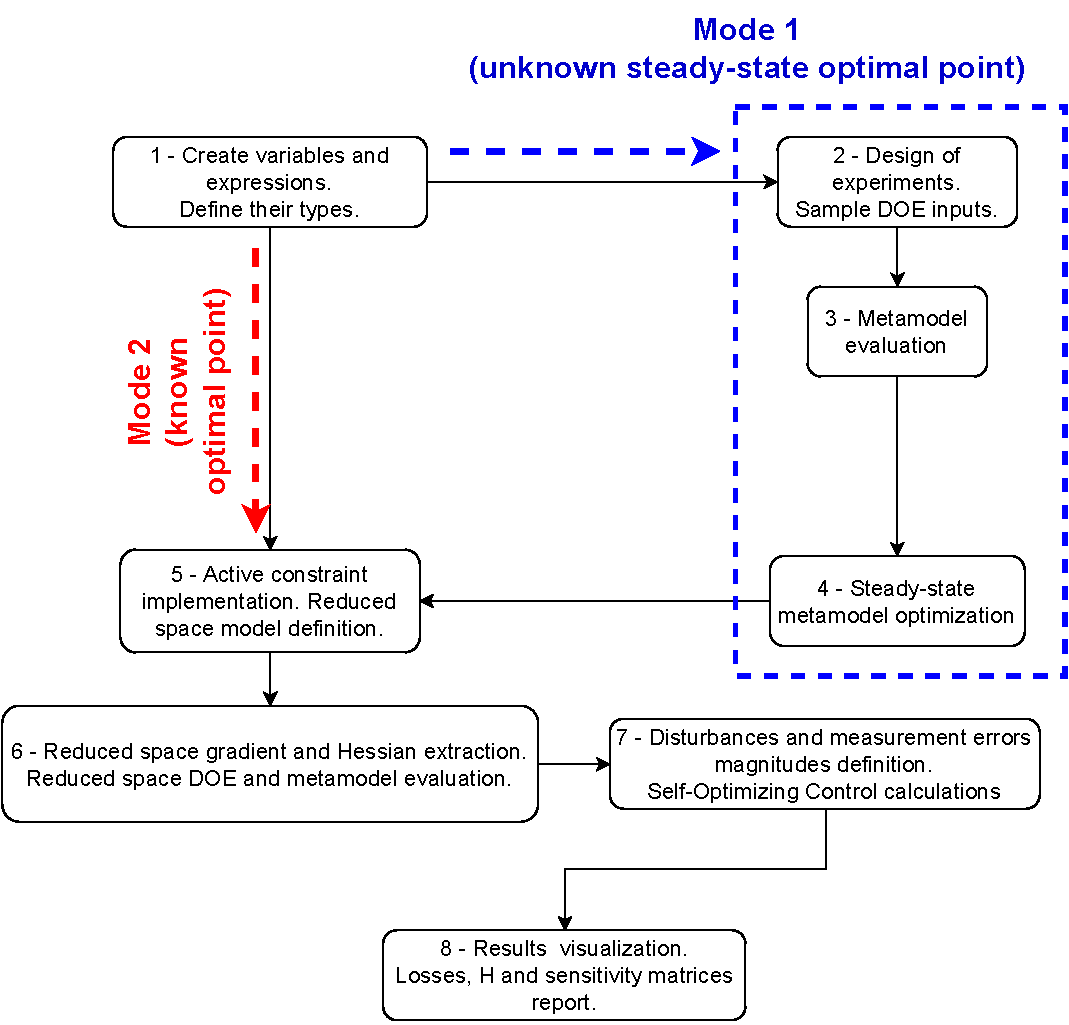
\includegraphics[width=1.0\textwidth]
    {metacontrol-workflow.pdf}}
    \fonte{Author}
    \label{fig:modemtc}
\end{figure}

\end{document}